\documentclass{report} % Change 'article' to 'report' to enable \chapter
\usepackage{booktabs}      % For \toprule, \midrule, and \bottomrule
\usepackage{caption}       % For better caption control
\usepackage{float}         % For [H] option in tables and figures
\usepackage{graphicx}      % For including images

\begin{document}

\chapter{Results}  % Now \chapter will work

\section{Evaluation Metrics}

The models' performance is evaluated using the following metrics:

\begin{itemize}
    \item \textbf{Accuracy:} Measures the proportion of correctly classified instances out of the total instances.
    \item \textbf{Precision:} Measures the proportion of true positive instances out of the total predicted positive instances.
    \item \textbf{Recall:} Measures the proportion of true positive instances out of the total actual positive instances.
    \item \textbf{F1 Score:} The harmonic mean of precision and recall, providing a single metric that balances both.
\end{itemize}

The table below summarizes the evaluation metrics for the models:

\begin{table}[H]
  \centering
  \caption{Evaluation Metrics for the Models}
  \vspace{0.5cm} % Adjust the space here if needed
  \begin{tabular}{@{\hskip 5pt} l @{\hskip 10pt} c @{\hskip 10pt} c @{\hskip 10pt} c @{\hskip 10pt} c @{\hskip 5pt}}
  \toprule
  \textbf{Model} & \textbf{Accuracy} & \textbf{Precision} & \textbf{Recall} & \textbf{F1 Score} \\
  \midrule
  VGG-16 Fine-tuned  & 0.997691 & 0.997712 & 0.997691 & 0.997691 \\
  VGG-16  & 0.993072 & 0.993093 & 0.993072 & 0.993072 \\
  CNN        & 0.969977 & 0.969997 & 0.969977 & 0.969977 \\
  \bottomrule
  \end{tabular}
\end{table}


\section{VGG-16 Fine-tuned}

\subsection{Training and Validation Loss}

\begin{figure}[H]
\centering
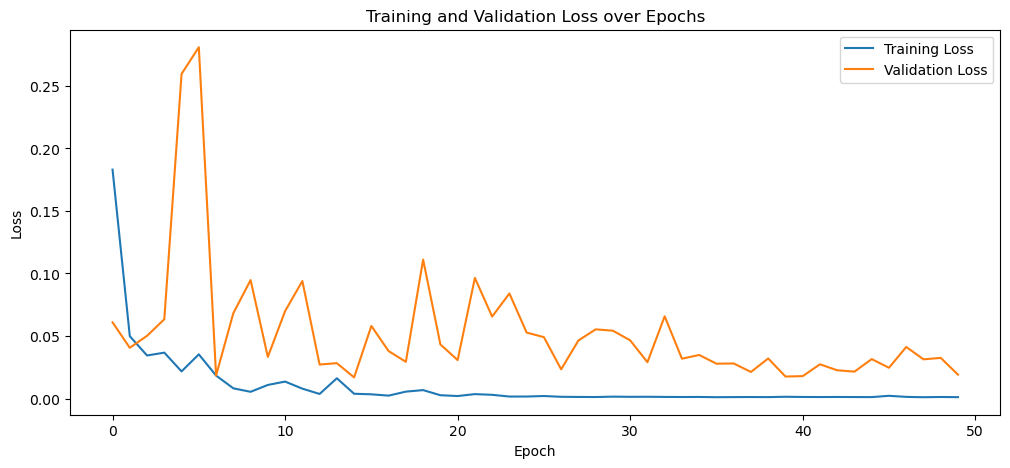
\includegraphics[width=0.8\textwidth]{train_val_loss_vgg16_uf.png}
\caption{Training and Validation Loss for VGG16 fine-tuned (last 3 layer)}
\end{figure}



\subsection{Training and Validation Accuracy}

\begin{figure}[H]
\centering
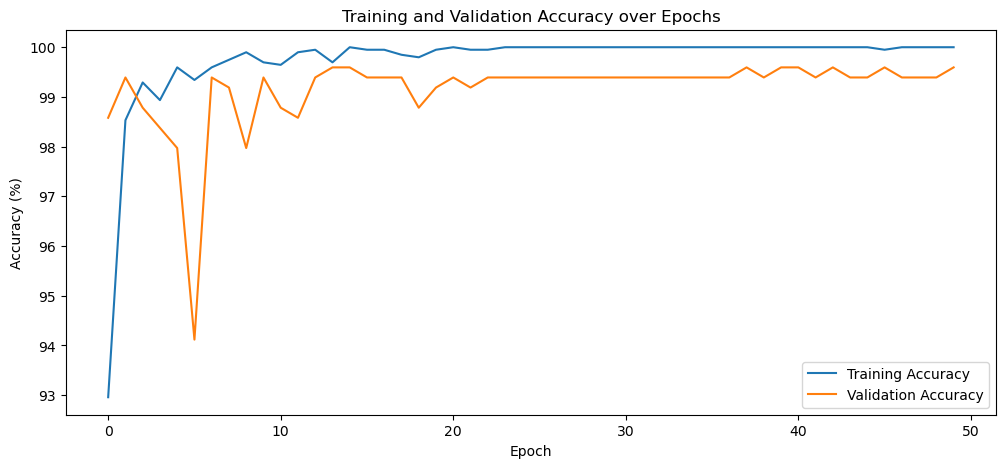
\includegraphics[width=0.8\textwidth]{train_val_acc_vgg16_uf.png}
\caption{Training and Validation Accuracy for VGG16 fine-tuned (last 3 layer)}
\end{figure}


\section{VGG16 with all layer convolutional  layer frozen}

\subsection{Training and Validation Loss}

\begin{figure}[H]
\centering
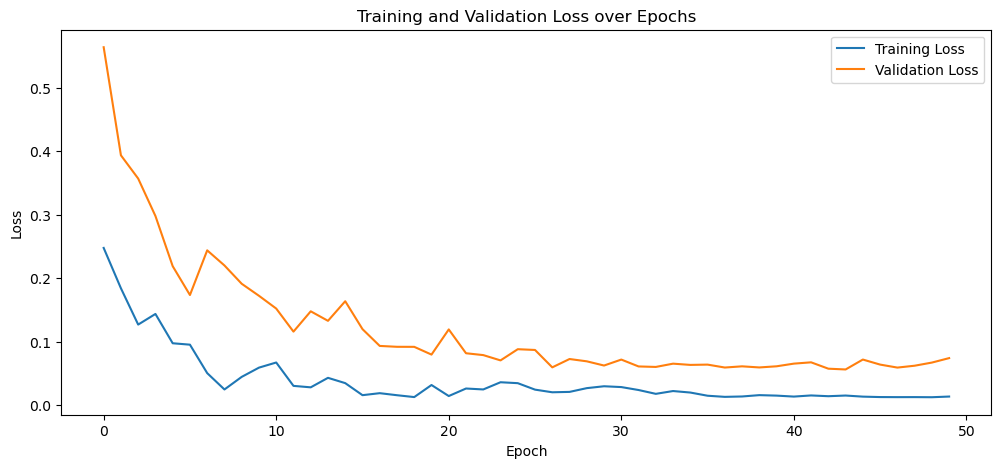
\includegraphics[width=0.8\textwidth]{train_val_err_vgg16.png}
\caption{Training and Validation Loss for VGG16 with Learning Rate Scheduler}
\end{figure}


\subsection{Training and Validation Accuracy}

\begin{figure}[H]
\centering
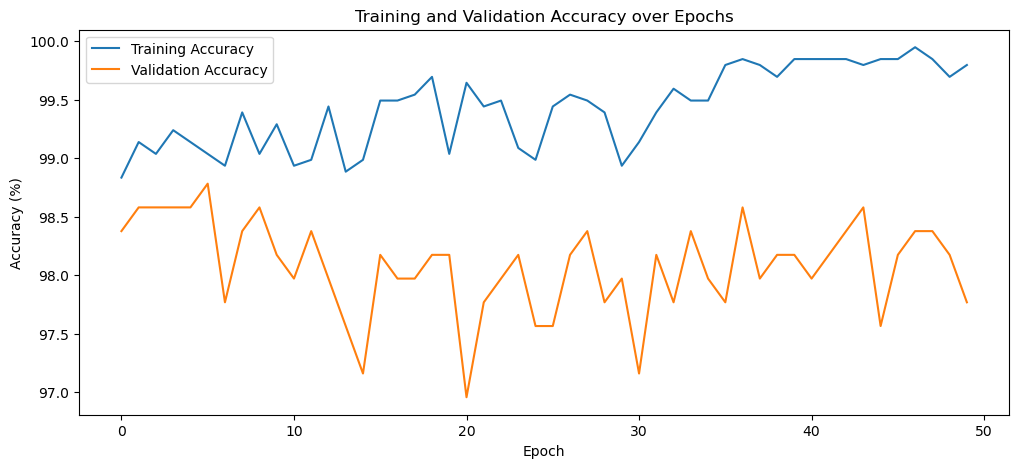
\includegraphics[width=0.8\textwidth]{train_val_acc_vgg16.png}
\caption{Training and Validation Accuracy for VGG16 with Learning Rate Scheduler}
\end{figure}


\section{Lightweight CNN}

\subsection{Training and Validation Loss}

\begin{figure}[H]
\centering
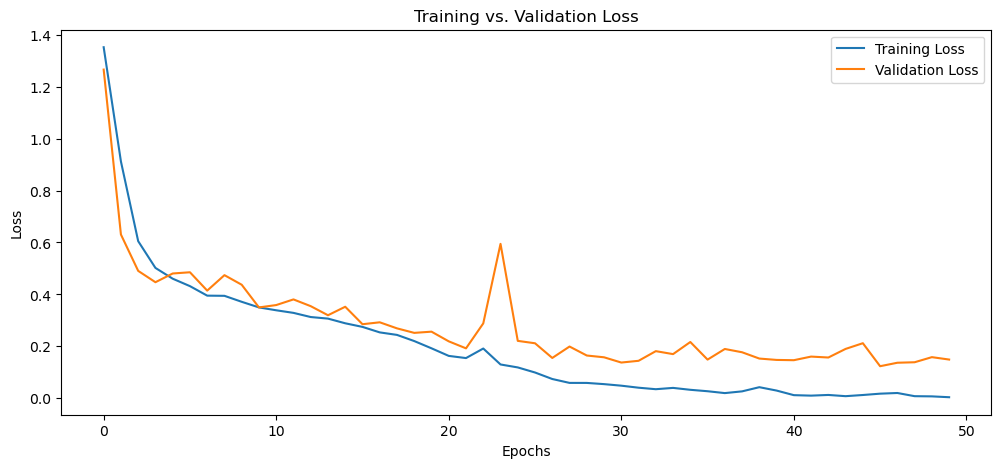
\includegraphics[width=0.8\textwidth]{train_valid_err_cnn.png}
\caption{Training and Validation Loss for Lightweight CNN}
\end{figure}


\subsection{Training and Validation Accuracy}

\begin{figure}[H]
\centering
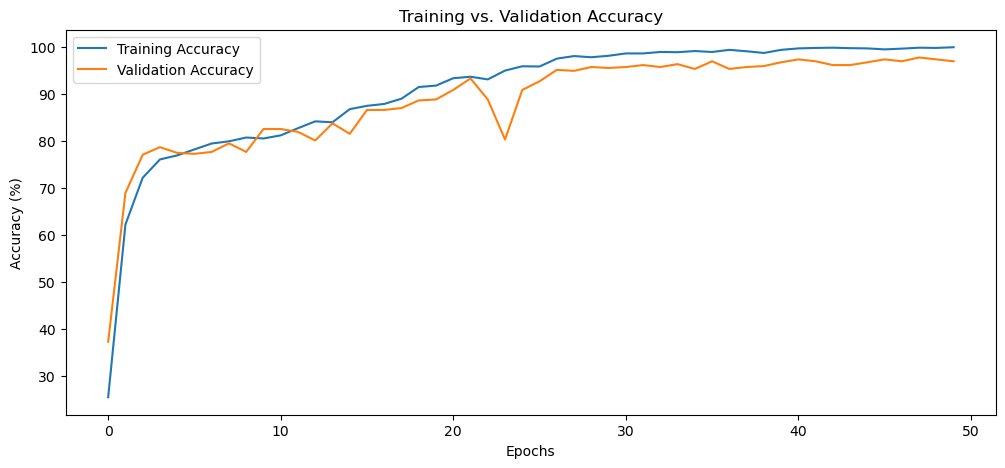
\includegraphics[width=0.8\textwidth]{train_valid_acc_cnn.png}
\caption{Training and Validation Accuracy for Lightweight CNN}
\end{figure}



\subsection{Confusion Matrix}



\begin{figure}[H]
\centering
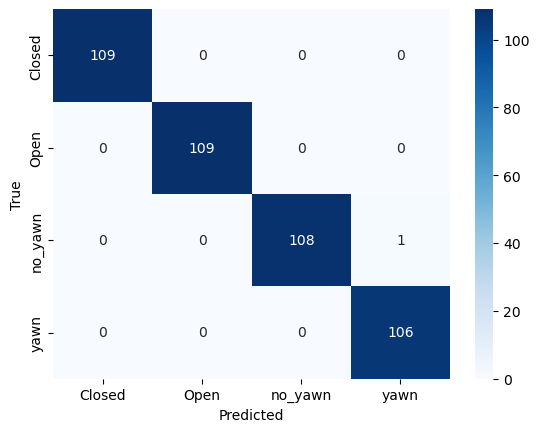
\includegraphics[width=0.8\textwidth]{vgg_16_unfreeze.png}
\caption{Confusion Matrix VGG16 with last 3 Convolutional Layers unfreezed}
\end{figure}

\begin{figure}[H]
  \centering
  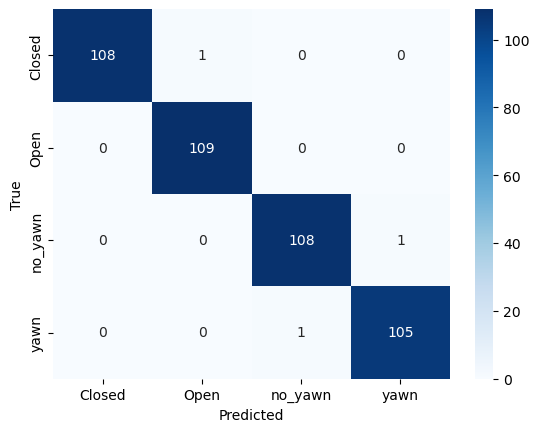
\includegraphics[width=0.8\textwidth]{vgg_16_freeze.png}
  \caption{Confusion Matrix for VGG16}
  \end{figure}

  \begin{figure}[H]
    \centering
    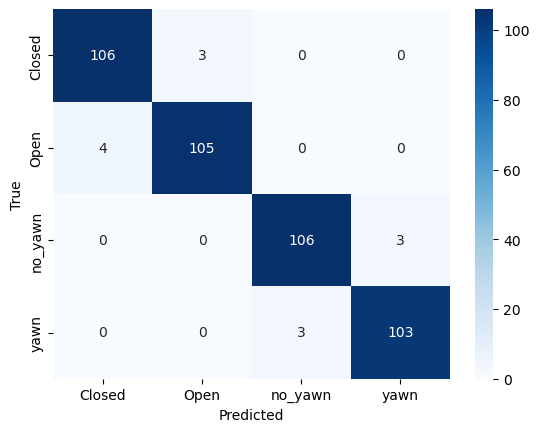
\includegraphics[width=0.8\textwidth]{conf_cnn.png}
    \caption{Confusion Matrix for Lightweight CNN}
    \end{figure}



\section{Conclusion}

The lightweight CNN model for detecting driver drowsiness and distraction demonstrates satisfactory performance metrics, including accuracy, precision, recall, and F1 score. The model's architecture balances computational efficiency and accuracy, making it suitable for real-time applications in driver monitoring systems. Future work will focus on implementing additional data augmentation techniques, hyperparameter tuning, and exploring more complex architectures or pre-trained models to further improve performance.

\begin{thebibliography}{9}
\bibitem{krizhevsky2012imagenet}
Krizhevsky, A., Sutskever, I., \& Hinton, G. E. (2012). ImageNet classification with deep convolutional neural networks. Advances in neural information processing systems, 25.

\bibitem{simonyan2014very}
Simonyan, K., \& Zisserman, A. (2014). Very deep convolutional networks for large-scale image recognition. arXiv preprint arXiv:1409.1556.

\bibitem{he2016deep}
He, K., Zhang, X., Ren, S., \& Sun, J. (2016). Deep residual learning for image recognition. In Proceedings of the IEEE conference on computer vision and pattern recognition (pp. 770-778).
\end{thebibliography}

\end{document}